\section{Multiclass Problem}
As I have seen, we have a different class distribution between DX\_bl and DX.
\begin{itemize}
	\item \textbf{DX\_bl} can be "CN", "SMC", "EMCI", "LMCI", and "AD". It indicates the screening diagnosis, i.e. the preliminary clinical judgment assigned during the first evaluation visit. It is a Screening diagnosis.
	\item \textbf{DX} can be "CN", "MCI", and "Dementia". It is instead the diagnosis assigned during the baseline visit (denoted by \textit{VISCODE} equal to "bl"), after a more in-depth clinical evaluation. 
\end{itemize}
"AD" and "Dementia" are the same thing despite the different names.

The acronym \textbf{SMC} refers to \textit{Subjective Memory Concern}, i.e., cognitively normal (CN) subjects reporting perceived memory issues. Since predicting a subjective perception from objective data is not meaningful. So I reassign it based on the value it has in DX.

\vspace{2mm}

Furthermore, we divide MCI into EMCI (Early MCI) and LMCI (Late MCI), assuming that DX\_bl values accurately distinguish EMCI and LMCI when DX equals MCI. This is because the division into EMCI and LMCI reflects the degree of cognitive impairment and the risk of progression to dementia.
\begin{itemize}
	\item \textbf{EMCI:} mild cognitive deficits, often detectable only with more sensitive tests. Lower or slower risk of progression to dementia.
	\item \textbf{LMCI:} more marked and evident impairment, greater impact on daily life. Higher risk of progression to Alzheimer's or other dementias.
\end{itemize}
Therefore, we decide to keep them in the diagnostic prediction.

\begin{figure}[H]
	\centering
	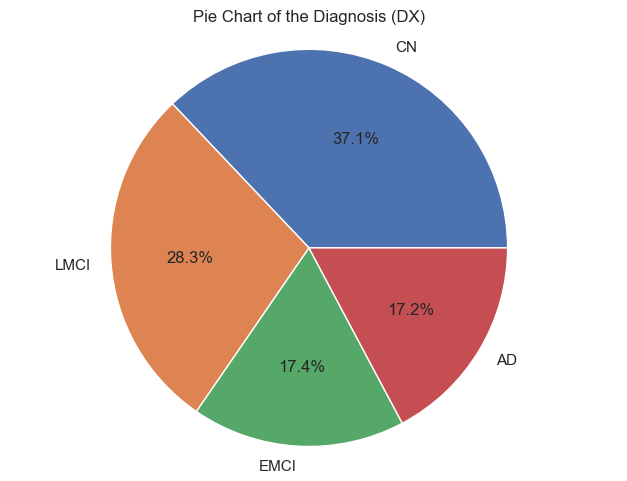
\includegraphics[width=0.48\textwidth]{images/DX_pie_chart.png}
	\label{fig:pie-chart-dx}
\end{figure}

\textbf{Ultimately, our target variable will be a modified version of the \textit{DX} column, which can now take on four values: "CN", "EMCI", "LMCI", and "AD." This makes our problem a multiclass problem.}

\newpage